\chapter{Обеспечение информационной безопасности в рамках Экосистемы OSTIS}
\chapauthortoc{Чертков В.~М.\\Захаров В.~В.}
\label{chapter_security}

\begin{SCn}
\begin{scnrelfromlist}{автор}
	\scnitem{Чертков В.~М.}
	\scnitem{Захаров В.~В.}
\end{scnrelfromlist}

\bigskip

\abstract{В главе рассмотрены методы и средства обеспечения безопасности традиционных информационных систем, особенности обеспечения информационной безопасности интеллектуальных систем нового поколения (см. \textit{Главу \ref{chapter_new_generation_systems}~\nameref{chapter_new_generation_systems}}) и принципы, лежащие в основе обеспечения информационной безопасности ostis-систем.}

\bigskip

\begin{scnrelfromlist}{подраздел}
	\scnitem{\ref{sec_security_specifics}~\nameref{sec_security_specifics}}
	\scnitem{\ref{sec_security_principles}~\nameref{sec_security_principles}}
\end{scnrelfromlist}

\bigskip

\begin{scnrelfromlist}{ключевой знак}
	\scnitem{Технология OSTIS}
	\scnitem{Экосистема OSTIS}
	\scnitem{ostis-система}
\end{scnrelfromlist}

\bigskip

\begin{scnrelfromlist}{ключевое понятие}
	\scnitem{база знаний ostis-системы}
\end{scnrelfromlist}

\bigskip

\begin{scnrelfromlist}{библиографическая ссылка}
	\scnitem{\scncite{Isoboev2022}}
	\scnitem{\scncite{Chastikova2022}}
	\scnitem{\scncite{Abdurahman2022}}
	\scnitem{\scncite{Ostrouh2020}}
	\scnitem{\scncite{Baranovich2011}}
	\scnitem{\scncite{Hoang2013}}
	\scnitem{\scncite{Golenkov2017a}}
	\scnitem{\scncite{Golenkov2019}}
	\scnitem{\scncite{Druzhinin2002}}
	\scnitem{\scncite{Dementiev2022}}
	\scnitem{\scncite{Skrypnikov2021}}
	\scnitem{\scncite{Sozinova2011}}
\end{scnrelfromlist}
\end{SCn}


\section*{Введение в \textit{Главу \ref{chapter_security}}}
Большое разнообразие моделей обеспечения информационной безопасности, всё возрастающий объем данных, которые необходимо анализировать для обнаружения атак на информационные системы, изменчивость методов атак и динамическое изменение защищаемых информационных систем, необходимость оперативного реагирования на атаки, нечеткость критериев обнаружения атак и выбора методов и средств реагирования на них, нехватка высококвалифицированных специалистов по защите влечет за собой потребность в использовании методов искусственного интеллекта для решения задач безопасности.

\section{Специфика обеспечения информационной безопасности интеллектуальных систем нового поколения}
\label{sec_security_specifics}
Информационную безопасность интеллектуальных систем следует рассматривать с двух точек зрения:
\begin{textitemize}
	\item с точки зрения применения \textit{искусственного интеллекта} в информационной безопасности;
	\item с точки зрения организации информационной безопасности в интеллектуальных системах.
\end{textitemize}

\textbf{Применение \textit{искусственного интеллекта} в информационной безопасности}

Следует отметить, что \textit{искусственный интеллект} активно применяется для мониторинга и анализа уязвимостей безопасности в сетях передачи информации (см. \scncite{Isoboev2022}). Система искусственного интеллекта позволяет машинам более эффективно выполнять поставленные задачи, такие как:

\begin{textitemize}
	\item визуальное восприятие, распознавание речи, принятие решений и перевод с одного языка на другой;
	
	\item \textit{обнаружение вторжений} --- \textit{искусственный интеллект} может обнаруживать сетевые атаки, заражения вредоносным программным обеспечением и другие киберугрозы;
	
	\item \textit{кибераналитика} --- \textit{искусственный интеллект} также используется для анализа больших данных с целью выявления закономерностей и аномалий в системе кибербезопасности организации с целью обнаружения не только известных, но и ещё неизвестных угроз;
	
	\item \textit{безопасная разработка программного обеспечения} --- \textit{искусственный интеллект} может помочь создать более безопасное программное обеспечение, предоставляя разработчикам обратную связь в режиме реального времени.
\end{textitemize}

При этом \textit{искусственный интеллект} используется не только для защиты, но и для нападения, например для эмуляции акустических, видео и других образов с целью обмана механизмов аутентификации и дальнейшей имперсонации, обман проверки человек или робот capcha.

В настоящее время можно определить следующие классы систем, в которых применяется \textit{искусственный интеллект} (см. \scncite{Skrypnikov2021}):

\begin{textitemize}
	\item UEBA (User and Entity Behavior Analytics) --- система анализа поведения субъектов (пользователей, программ, агентов) на предмет обнаружения нестандартного поведения и использования их для обнаружения потенциальных угроз с использованием шаблонов угроз (паттернов);
	\item TIP (Threat Intelligence Platform) --- платформы раннего обнаружения угроз на основе сбора и анализа информации индикаторов компрометации и реагирования на них. Применение методов машинного обучения повышает эффективность обнаружения неизвестных угроз на ранних этапах;
	\item EDR (Endpoint Detection and Response) --- системы обнаружения атак оперативного реагирования на конечных точках компьютерной сети. Могут обнаруживать вредоносные программы, автоматически классифицировать угрозы и самостоятельно реагировать на них;
	\item SIEM (Security Information and EventManagement) --- системы сбора и анализа информации о событиях безопасности от сетевых устройств и приложений в реальном времени и оповещения;
	\item NDR (Network Detection and Response) --- системы обнаружения атак на сетевом уровне и оперативного реагирования на них. \textit{Искусственный интеллект} использует накопленную статистику и базу знаний об угрозах;
	\item SOAR (Security Orchestration and Automated Response) --- системы, позволяющие выявлять угрозы информационной безопасности и автоматизировать реагирование на инциденты. В решениях данного типа, в отличие от SIEM-систем, \textit{Искусственный интеллект} помогает не только проводить анализ, но и автоматически реагировать надлежащим образом на выявленные угрозы;
	\item Средства защиты приложений (Application Security) --- системы, позволяющие определять угрозы безопасности прикладных приложений, управлять процессом мониторинга и устранения таких угроз;
	\item Антифрод (Antifraud) --- платформы в режиме реального времени обнаруживают угрозы в бизнес-процессах и мошеннические операции. \textit{Искусственный интеллект} используется для определения отклонений от идентифицированных бизнес-процессов с целью выявления вторжений или уязвимости процессов и повышает адаптивность к изменению логики и метрик бизнес-процессов.
\end{textitemize}


В работе \scncite{Chastikova2022} предложена методика построения нейроиммунной системы анализа инцидентов информационной безопасности, объединяющей модули сбора и хранения (сжатия) данных, модуль анализа и корреляции событий информационной безопасности и подсистемы обнаружения сетевых атак на основе сверточных нейронных сетей. Использование технологий машинного обучения в информационной безопасности создает узкие места и системные уязвимости, которые можно использовать, и имеет следующие недостатки (см. \scncite{Abdurahman2022}):

\begin{textitemize}
	\item наборы данных, которые должны быть сформированы из значительного количества входных выборок, что требует много времени и ресурсов;
	\item требуется огромное количество ресурсов, включая память, данные и вычислительную мощность;
	\item частые ложные срабатывания, которые нарушают работу и в целом снижают эффективность таких систем;
	\item организованные атаки на основе \textit{искусственного интеллекта} (семантические вирусы).
\end{textitemize}

\textbf{Организация информационной безопасности в интеллектуальных системах нового поколения}

Определим цели обеспечения информационной безопасности систем нового поколения.

Из монографии \scncite{Ostrouh2020} \textbf{\textit{Целями обеспечения информационной безопасности традиционных интеллектуальных систем}} являются:

\begin{textitemize}
	\item обеспечение конфиденциальности информации в соответствии с проведенной классификацией;
	\item обеспечение целостности информации на всех этапах, связанных с нею процессов (создание, обработка, хранение, передача и уничтожение) при предоставлении публичных услуг;
	\item обеспечение своевременной доступности информации при предоставлении публичных услуг;
	\item обеспечение наблюдаемости, направленной на фиксирование любой деятельности пользователей и процессов;
	\item обеспечение аутентичности и невозможности отказа от транзакций и действий, производимых участниками предоставления публичных услуг;
	\item учет всех процессов и событий, связанных с вводом, обработкой, хранением, предоставлением и уничтожением данных.
\end{textitemize}

Следует отметить так как интеллектуальные системы нового поколения будут взаимодействовать с подобными себе системами понимая при этом, о чем осуществляется запрос, то цели обеспечения будут выглядеть по-другому. \textit{Целями обеспечения информационной безопасности интеллектуальных систем нового поколения} являются:

\begin{textitemize}
	\item обеспечение сохранности семантической совместимости информации;
	\item защита достоверности и целостности информации;
	\item обеспечение доступности информации на разных уровнях интеллектуальной системы;
	\item минимизация ущерба от событий, несущих угрозу информационной безопасности.
\end{textitemize}

В настоящее время разработаны классические подходы и принципы обеспечения безопасности баз знаний (данных), интерфейсов связи (обмена информацией) между компонентами интеллектуальных систем такие, как шифрование передаваемых данных, фильтрация ненужного (избыточного) контента и политика разграничения доступа к данным.

Система обеспечения информационной безопасности должна создаваться на следующих принципах:

\begin{textitemize}
	\item \textit{Принцип равнопрочности} --- означает обеспечение защиты оборудования, программного обеспечения и системы управления от всех видов угроз;
	\item \textit{Принцип непрерывности} --- предусматривает непрерывное обеспечение безопасности информационных ресурсов системы для непрерывного предоставления публичных услуг;
	\item \textit{Принцип разумной достаточности} --- означает применение таких мер и средств защиты, которые являются разумными, рациональными и затраты на которые, не превышают стоимости последствий нарушения информационной безопасности;
	\item \textit{Принцип комплексности} --- для обеспечения безопасности во всем многообразии структурных элементов, угроз и каналов несанкционированного доступа должны применяться все виды и формы защиты в полном объеме;
	\item \textit{Принцип комплексной проверки} --- заключается в проведении специальных исследований и проверок, специального инженерного анализа оборудования, верификационных исследований программных средств. Должен осуществляться непрерывный мониторинг аварийных сообщений и параметров ошибок, постоянно должно выполняться тестирование аппаратного и программного оборудования, а также контроль целостности программных средств, как при загрузке программных средств, так и в процессе функционирования;
	\item \textit{Принцип надежности} --- методы, средства и формы защиты должны надежно перекрывать все пути проникновения и возможные каналы утечки информации, для этого допускается дублирование средств и мер безопасности;
	\item \textit{Принцип универсальности} --- меры безопасности должны перекрывать пути угроз независимо от места их возможного воздействия;
	\item \textit{Принцип плановости} --- планирование должно осуществляться путем разработки детальных планов действий по обеспечению информационной защищенности всех компонент системы предоставления публичных услуг;
	\item \textit{Принцип централизованного управления} --- в рамках определенной структуры должна обеспечиваться организованно-функциональная самостоятельность процесса обеспечения безопасности при предоставлении публичных услуг;
	\item \textit{Принцип целенаправленности} --- необходимо защищать то, что должно защищаться в интересах конкретной цели;
	\item \textit{Принцип активности} --- защитные меры обеспечения безопасности в работе процесса предоставления услуг должны претворяться в жизнь с достаточной степенью настойчивости;
	\item \textit{Принцип квалификации обслуживающего персонала} --- обслуживание оборудования должно осуществляться сотрудниками, подготовленными не только в вопросах эксплуатации техники, но и в технических вопросах обеспечения безопасности информации;
	\item \textit{Принцип ответственности} --- ответственность за обеспечение информационной безопасности должна быть ясно установлена, передана соответствующему персоналу и утверждена всеми участниками в рамках процесса обеспечения информационной безопасности.
\end{textitemize}

\section{Принципы, лежащие в основе обеспечения информационной безопасности ostis-систем}
\label{sec_security_principles}

\begin{figure}[H]
	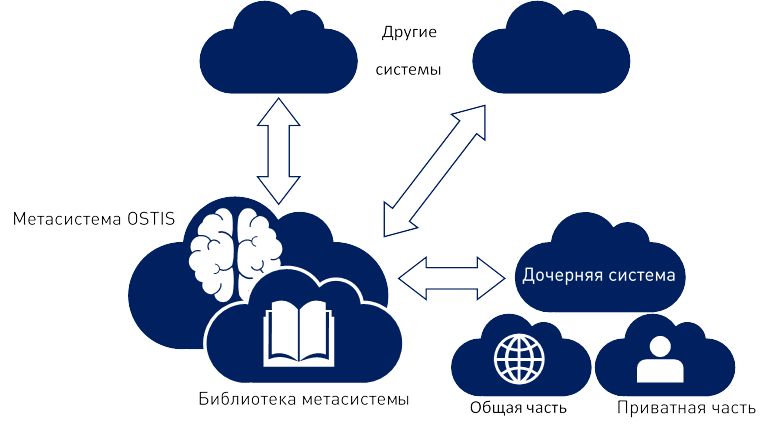
\includegraphics[scale=0.9]{images/part7/chapter_security/ecosystem_security.png}
	\caption{Рисунок. Архитектура Экосистемы OSTIS}
	\label{fig:ecosystem_security}
\end{figure}

Структура \textit{Экосистемы OSTIS} детально рассмотрена в \textit{Главе \ref{chapter_ecosystem}~\nameref{chapter_ecosystem}}.  В \textit{Экосистеме OSTIS} требуется организация обеспечения информационной безопасности на каждом из уровней: обмен данными, права доступа к данным, аутентификация клиентов Экосистемы, шифрование данных, получение данных из открытых источников, обеспечение достоверности и целостности хранимых и передаваемых данных, контроль за нарушением связей в базе знаний.

Важно отметить, что информационная безопасность тесно связана с архитектурой построенной системы: грамотно спроектированная и хорошо управляемая система сложнее поддается взлому. Поэтому очень важно разрабатывать систему информационной безопасности на этапе проектирования архитектуры и структуры будущей интеллектуальной системы нового поколения.

\textit{Экосистема OSTIS} --- это сообщество, где происходит взаимодействие \textit{ostis-систем} и пользователей, где должны быть установлены правила, которые должны контролироваться. Нельзя допускать противоправные и дестабилизирующие действия со стороны всех участников сообщества. Пользователь не может на прямую осуществлять взаимодействия с другими \textit{ostis-системами}, а только через персонального агента. Этот агент хранит все персональные данные пользователя и доступ к ним должен быть ограничен.

В \textit{Экосистеме OSTIS} все агенты должны быть идентифицированы. Следует отметить, что персональный агент пользователя в Экосистеме решает проблему идентификации самого пользователя.

В рассмотренной \textit{Экосистеме OSTIS} требуется организация обеспечения информационной безопасности на каждом из уровней взаимодействия: обмен данными, права доступа к данным, аутентификация клиентов Экосистемы, шифрование данных, получение данных из открытых источников, обеспечение достоверности и целостности хранимых и передаваемых данных, контроль за нарушением связей в базе знаний, отслеживание уязвимостей в системе.

\begin{SCn}
	\scnheader{угроза в ostis-системе}
	\scnsuperset{нарушение конфиденциальности информации}
	\begin{scnindent}
		\scnexplanation{блокирование доступа к системе, отдельным ее компонентам, функциям или информации, а также невозможность своевременного получения информации (неприемлемые задержки в получении информации)}
	\end{scnindent}
	
	\scnsuperset{нарушение целостности информации}
	\begin{scnindent}
		\scnexplanation{несанкционированное или ошибочное изменение, искажение или уничтожение информации, а также несанкционированные воздействия на технические и программные средства обработки информации}
	\end{scnindent}
	
	\scnsuperset{нарушение доступности}
	\begin{scnindent}
		\scnexplanation{блокирование доступа к системе, отдельным ее компонентам, функциям или информации, а также невозможность своевременного получения информации (неприемлемые задержки в получении информации)}
	\end{scnindent}

	\scnsuperset{нарушение семантической совместимости}
	\begin{scnindent}
		\scnexplanation{нарушение общности понятий и в общности базовых знаний}
	\end{scnindent}
	
	\scnsuperset{разрушения семантики баз знаний (семантические вирусы)}
	\begin{scnindent}
		\scnexplanation{подмена или удаление узлов и связей между ними в базе знаний}
	\end{scnindent}
	
	\scnsuperset{избыточный объем входящей информации}
	
	\scnsuperset{нарушение неотказуемости}
	\begin{scnindent}
		\scnexplanation{выдача несанкционированных действий за легальные, а также сокрытие или подмена информации о действиях субъектов}
	\end{scnindent}
	
	\scnsuperset{нарушение подотчетности}
	\begin{scnindent}
		\scnexplanation{несанкционированное или ошибочное изменение, искажение или уничтожение информации о выполнении действий субъектом}
	\end{scnindent}
	
	\scnsuperset{нарушение подлинности (аутентичности)}
	\begin{scnindent}
		\scnexplanation{выполнение действий в системе от имени другого лица или выдача недостоверных ресурсов (в том числе и данных) за подлинные}
	\end{scnindent}
	
	\scnsuperset{нарушение достоверности}
	\begin{scnindent}
		\scnexplanation{преднамеренное или непреднамеренное предоставление и использование ошибочной (неправильной) или неактуальной (на конкретный момент времени) информации, а также выполнение процедур в нарушении регламента (протокола)}
	\end{scnindent}
\end{SCn}

Представим основные направления обеспечения информационной безопасности \textit{ostis-систем} по предупреждению возникающих угроз:

\begin{textitemize}
	\item ограничение информационного трафика, анализируемого интеллектуальной системой;
	\item политика разграничении доступа к базе знаний;
	\item связность;
	\item введение семантической метрики;
	\item семантическая совместимость;
	\item активность.
\end{textitemize}

Следует отметить, что на этапе проектирования самой \textit{Технологии OSTIS} уже были заложены основные принципы обеспечения информационной безопасности, в рамках проектирования отдельных компонентов системы. Так уже изначально поддержка семантической совместимости и связности обеспечиваются в \textit{ostis-системах} за счет способности системы обнаруживать вредоносные процессы в базе знаний.

\textbf{Ограничение информационного трафика, анализируемого интеллектуальной системой}

Экспоненциальный рост объема информации, циркулирующей в информационных потоках и ресурсах в условиях вполне определенных количественных ограничений на возможности средств ее восприятия, хранения, передачи и преобразования формирует новый класс угроз информационной безопасности, характеризуемых избыточностью совокупного входящего информационного трафика интеллектуальных систем.

В результате переполнение информационных ресурсов интеллектуальной системы избыточной информацией может спровоцировать распространения искаженной (деструктивной семантической) информации. Общая методология защиты интеллектуальных систем от избыточного информационного трафика осуществляется посредством использования аксиологических фильтров, реализующих функции численной оценки ценности поступающей информации, отбора наиболее ценной и отсеивания (фильтрации) менее ценной (бесполезной или вредной) с использованием вполне определенных критериев.

Следует также выделить в отдельную категорию угроз информационной безопасности активные средства разрушения семантики баз знаний (семантические вирусы) (см. \scncite{Baranovich2011}).

\textbf{Политика разграничении доступа к базе знаний}

Мандатная политика безопасности (MAC --- mandatory access control) основывается на мандатном (принудительном) разграничении доступа, определяющемся четырьмя условиями: все субъекты и объекты системы идентифицируются; задается решетка уровней безопасности информации; каждому объекту системы присваивается уровень безопасности, определяющий важность содержащейся в нем информации; каждому субъекту системы присваивается уровень доступа, определяющий уровень доверия к нему в интеллектуальной системе. Кроме того, мандатная политика имеет более высокую степень надёжности. Реализация данной политики основывается на разработанном алгоритме определения согласованных уровней безопасности всех элементов онтологии.

Так как семантические базы знаний в отличие от реляционной базы данных позволяют выполнять правила для получения логических выводов, то для обеспечения безопасности данных актуальным является разработка алгоритмов и методов, с помощью которых можно будет получать только данные, имеющие уровни безопасности меньше уровней доступа субъектов их запросивших (см. \scncite{Hoang2013}).

\textbf{Связность}

Вся информация, хранимая в семантической памяти интеллектуальной системы, систематизирована в виде единой базы знаний. К такой информации относятся непосредственно обрабатываемые знания, интерпретируемые программы, формулировки решаемых задач, планы и протоколы решения задач, информация о пользователях, описание синтаксиса и семантики внешних языков, описание пользовательского интерфейса и многое другое (см. \scncite{Golenkov2017a}). В информационной базе знаний между фрагментами информации (единицами информации) должна быть предусмотрена возможность установления связей различного типа. Прежде всего, эти связи могут характеризовать отношения между информационными единицами. Нарушение связей приводит к неправильному логическому выводу, либо к получению ложных знаний, либо к несовместимости знаний в базе. Данное направление более детально рассмотрено в \textit{Главе \ref{chapter_kb_design} \nameref{chapter_kb_design}}.

\textbf{Введение семантической метрики}

На множестве информационных единиц в некоторых случаях полезно задавать отношение, характеризующее семантическую близость информационных единиц, то есть силу ассоциативной связи между информационными единицами (см. \scncite{Dementiev2022}). Его можно было бы назвать отношением релевантности для информационных единиц. Такое отношение дает возможность выделять в информационной базе знаний некоторые типовые ситуации. Отношение релевантности при работе с информационными единицами позволяет находить знания, близкие к уже найденным.

\textbf{Семантическая совместимость}

Внутренняя семантическая совместимость между компонентами интеллектуальной компьютерной системы (максимально возможное введение общих, совпадающих понятий для различных фрагментов хранимой базы знаний), являющаяся формой конвергенции и глубокой интеграции внутри интеллектуальной компьютерной системы для различного вида знаний и различных моделей решения задач, что обеспечивает эффективную реализацию мультимодальности интеллектуальной компьютерной системы. Внешняя семантическая совместимость между различными интеллектуальными компьютерными системами, выражающаяся не только в общности используемых понятий, но и в общности базовых знаний и являющаяся необходимым условием обеспечения высокого уровня социализации интеллектуальных компьютерных систем (см. \scncite{Golenkov2019}). Более подробно рассмотрено в \textit{Главе \ref{chapter_new_generation_systems} \nameref{chapter_new_generation_systems}}.

\textbf{Активность}

В интеллектуальной системе для актуализации тех или иных действий способствуют знания, имеющиеся в этой системе. Таким образом, выполнение активностей в интеллектуальной системе должно инициироваться текущим состоянием информационной базы знаний. Появление в базе фактов или описаний событий, установление связей может стать источником активности системы (см. \scncite{Druzhinin2002}). В том числе преднамеренное искажение информации и связей может стать источником преднамеренного искажения информации.

Для интеллектуальных систем нового поколения можно выделить ряд аспектов, в рамках которых требуется работка новых алгоритмов и методов обеспечения информационной безопасности в дополнении к существующим механизмам:

\begin{textitemize}
	\item многоуровневый доступ к отдельным частям базы знаний, так как информация бывает общедоступной, персональной, конфиденциальной;
	\item мониторинг изменений значений слов с течением времени, а также значений перевода с иностранного языка которые могут влиять на принимаемые решения;
	\item защиты от несанкционированного использования путем применения криптосемантических шифров;
	\item постоянный мониторинг уязвимостей в системе;
	\item протоколирование действий (взаимодействий) системы.
\end{textitemize}

Для решения поставленных задач может быть применена экспертная \textit{ostis-система}, способная обеспечить обнаружение злоупотреблений и аномалий в поведении всех участников \textit{Экосистемы OSTIS} на основе постоянного мониторинга и введения протоколов взаимодействий участников.

Создание и применение экспертных систем является одним из важных этапов развития информационных технологий и информационной безопасности (см. \scncite{Sozinova2011}). Соответственно, решение задач обеспечения информационной безопасности может быть получено на базе использования экспертных систем:

\begin{textitemize}
	\item появляется возможность решения сложных задач с привлечением нового, специально разработанного для этих целей математического аппарата (семантических сетей, фреймов, нечеткой логики);
	\item применение экспертных систем позволяет значительно повысить эффективность, качество и оперативность решений за счет аккумуляции знаний;
\end{textitemize}

\section*{Заключение к Главе~\ref{chapter_security}}
Для эффективной информационной защиты системы на современном этапе необходим симбиоз традиционных технологий, и технологий, реализуемых в рамках \textit{OSTIS}. Также следует отметить, что обеспечение информационной безопасности на базе \textit{Технологии OSTIS} осуществляется значительно проще, потому что многие аспекты уже реализованы на этапе проектирования самой технологии. Важно отметить, что интеллектуальная информационная система нового поколения --- это самостоятельный субъект, который может сам осознанно, целенаправленно и постоянно заботиться о себе, в том числе о своей собственной безопасности.


%%%%%%%%%%%%%%%%%%%%%%%%% referenc.tex %%%%%%%%%%%%%%%%%%%%%%%%%%%%%%
% sample references
% %
% Use this file as a template for your own input.
%
%%%%%%%%%%%%%%%%%%%%%%%% Springer-Verlag %%%%%%%%%%%%%%%%%%%%%%%%%%
%
% BibTeX users please use
% \bibliographystyle{}
% \bibliography{}
%
\biblstarthook{In view of the parallel print and (chapter-wise) online publication of your book at \url{www.springerlink.com} it has been decided that -- as a genreral rule --  references should be sorted chapter-wise and placed at the end of the individual chapters. However, upon agreement with your contact at Springer you may list your references in a single seperate chapter at the end of your book. Deactivate the class option \texttt{sectrefs} and the \texttt{thebibliography} environment will be put out as a chapter of its own.\\\indent
References may be \textit{cited} in the text either by number (preferred) or by author/year.\footnote{Make sure that all references from the list are cited in the text. Those not cited should be moved to a separate \textit{Further Reading} section or chapter.} If the citatiion in the text is numbered, the reference list should be arranged in ascending order. If the citation in the text is author/year, the reference list should be \textit{sorted} alphabetically and if there are several works by the same author, the following order should be used:
\begin{enumerate}
\item all works by the author alone, ordered chronologically by year of publication
\item all works by the author with a coauthor, ordered alphabetically by coauthor
\item all works by the author with several coauthors, ordered chronologically by year of publication.
\end{enumerate}
The \textit{styling} of references\footnote{Always use the standard abbreviation of a journal's name according to the ISSN \textit{List of Title Word Abbreviations}, see \url{http://www.issn.org/en/node/344}} depends on the subject of your book:
\begin{itemize}
\item The \textit{two} recommended styles for references in books on \textit{mathematical, physical, statistical and computer sciences} are depicted in ~\cite{science-contrib, science-online, science-mono, science-journal, science-DOI} and ~\cite{phys-online, phys-mono, phys-journal, phys-DOI, phys-contrib}.
\item Examples of the most commonly used reference style in books on \textit{Psychology, Social Sciences} are~\cite{psysoc-mono, psysoc-online,psysoc-journal, psysoc-contrib, psysoc-DOI}.
\item Examples for references in books on \textit{Humanities, Linguistics, Philosophy} are~\cite{humlinphil-journal, humlinphil-contrib, humlinphil-mono, humlinphil-online, humlinphil-DOI}.
\item Examples of the basic Springer style used in publications on a wide range of subjects such as \textit{Computer Science, Economics, Engineering, Geosciences, Life Sciences, Medicine, Biomedicine} are ~\cite{basic-contrib, basic-online, basic-journal, basic-DOI, basic-mono}. 
\end{itemize}
}

\begin{thebibliography}{99.}%
% and use \bibitem to create references.
%
% Use the following syntax and markup for your references if 
% the subject of your book is from the field 
% "Mathematics, Physics, Statistics, Computer Science"
%
% Contribution 
\bibitem{science-contrib} Broy, M.: Software engineering --- from auxiliary to key technologies. In: Broy, M., Dener, E. (eds.) Software Pioneers, pp. 10-13. Springer, Heidelberg (2002)
%
% Online Document
\bibitem{science-online} Dod, J.: Effective substances. In: The Dictionary of Substances and Their Effects. Royal Society of Chemistry (1999) Available via DIALOG. \\
\url{http://www.rsc.org/dose/title of subordinate document. Cited 15 Jan 1999}
%
% Monograph
\bibitem{science-mono} Geddes, K.O., Czapor, S.R., Labahn, G.: Algorithms for Computer Algebra. Kluwer, Boston (1992) 
%
% Journal article
\bibitem{science-journal} Hamburger, C.: Quasimonotonicity, regularity and duality for nonlinear systems of partial differential equations. Ann. Mat. Pura. Appl. \textbf{169}, 321--354 (1995)
%
% Journal article by DOI
\bibitem{science-DOI} Slifka, M.K., Whitton, J.L.: Clinical implications of dysregulated cytokine production. J. Mol. Med. (2000) doi: 10.1007/s001090000086 
%
\bigskip

% Use the following (APS) syntax and markup for your references if 
% the subject of your book is from the field 
% "Mathematics, Physics, Statistics, Computer Science"
%
% Online Document
\bibitem{phys-online} J. Dod, in \textit{The Dictionary of Substances and Their Effects}, Royal Society of Chemistry. (Available via DIALOG, 1999), 
\url{http://www.rsc.org/dose/title of subordinate document. Cited 15 Jan 1999}
%
% Monograph
\bibitem{phys-mono} H. Ibach, H. L\"uth, \textit{Solid-State Physics}, 2nd edn. (Springer, New York, 1996), pp. 45-56 
%
% Journal article
\bibitem{phys-journal} S. Preuss, A. Demchuk Jr., M. Stuke, Appl. Phys. A \textbf{61}
%
% Journal article by DOI
\bibitem{phys-DOI} M.K. Slifka, J.L. Whitton, J. Mol. Med., doi: 10.1007/s001090000086
%
% Contribution 
\bibitem{phys-contrib} S.E. Smith, in \textit{Neuromuscular Junction}, ed. by E. Zaimis. Handbook of Experimental Pharmacology, vol 42 (Springer, Heidelberg, 1976), p. 593
%
\bigskip
%
% Use the following syntax and markup for your references if 
% the subject of your book is from the field 
% "Psychology, Social Sciences"
%
%
% Monograph
\bibitem{psysoc-mono} Calfee, R.~C., \& Valencia, R.~R. (1991). \textit{APA guide to preparing manuscripts for journal publication.} Washington, DC: American Psychological Association.
%
% Online Document
\bibitem{psysoc-online} Dod, J. (1999). Effective substances. In: The dictionary of substances and their effects. Royal Society of Chemistry. Available via DIALOG. \\
\url{http://www.rsc.org/dose/Effective substances.} Cited 15 Jan 1999.
%
% Journal article
\bibitem{psysoc-journal} Harris, M., Karper, E., Stacks, G., Hoffman, D., DeNiro, R., Cruz, P., et al. (2001). Writing labs and the Hollywood connection. \textit{J Film} Writing, 44(3), 213--245.
%
% Contribution 
\bibitem{psysoc-contrib} O'Neil, J.~M., \& Egan, J. (1992). Men's and women's gender role journeys: Metaphor for healing, transition, and transformation. In B.~R. Wainrig (Ed.), \textit{Gender issues across the life cycle} (pp. 107--123). New York: Springer.
%
% Journal article by DOI
\bibitem{psysoc-DOI}Kreger, M., Brindis, C.D., Manuel, D.M., Sassoubre, L. (2007). Lessons learned in systems change initiatives: benchmarks and indicators. \textit{American Journal of Community Psychology}, doi: 10.1007/s10464-007-9108-14.
%
%
% Use the following syntax and markup for your references if 
% the subject of your book is from the field 
% "Humanities, Linguistics, Philosophy"
%
\bigskip
%
% Journal article
\bibitem{humlinphil-journal} Alber John, Daniel C. O'Connell, and Sabine Kowal. 2002. Personal perspective in TV interviews. \textit{Pragmatics} 12:257--271
%
% Contribution 
\bibitem{humlinphil-contrib} Cameron, Deborah. 1997. Theoretical debates in feminist linguistics: Questions of sex and gender. In \textit{Gender and discourse}, ed. Ruth Wodak, 99--119. London: Sage Publications.
%
% Monograph
\bibitem{humlinphil-mono} Cameron, Deborah. 1985. \textit{Feminism and linguistic theory.} New York: St. Martin's Press.
%
% Online Document
\bibitem{humlinphil-online} Dod, Jake. 1999. Effective substances. In: The dictionary of substances and their effects. Royal Society of Chemistry. Available via DIALOG. \\
http://www.rsc.org/dose/title of subordinate document. Cited 15 Jan 1999
%
% Journal article by DOI
\bibitem{humlinphil-DOI} Suleiman, Camelia, Daniel C. O'Connell, and Sabine Kowal. 2002. `If you and I, if we, in this later day, lose that sacred fire...': Perspective in political interviews. \textit{Journal of Psycholinguistic Research}. doi: 10.1023/A:1015592129296.
%
%
%
\bigskip
%
%
% Use the following syntax and markup for your references if 
% the subject of your book is from the field 
% "Computer Science, Economics, Engineering, Geosciences, Life Sciences"
%
%
% Contribution 
\bibitem{basic-contrib} Brown B, Aaron M (2001) The politics of nature. In: Smith J (ed) The rise of modern genomics, 3rd edn. Wiley, New York 
%
% Online Document
\bibitem{basic-online} Dod J (1999) Effective Substances. In: The dictionary of substances and their effects. Royal Society of Chemistry. Available via DIALOG. \\
\url{http://www.rsc.org/dose/title of subordinate document. Cited 15 Jan 1999}
%
% Journal article by DOI
\bibitem{basic-DOI} Slifka MK, Whitton JL (2000) Clinical implications of dysregulated cytokine production. J Mol Med, doi: 10.1007/s001090000086
%
% Journal article
\bibitem{basic-journal} Smith J, Jones M Jr, Houghton L et al (1999) Future of health insurance. N Engl J Med 965:325--329
%
% Monograph
\bibitem{basic-mono} South J, Blass B (2001) The future of modern genomics. Blackwell, London 
%
\end{thebibliography}
